\documentclass[border=4pt]{standalone}
\usepackage{amsmath,amssymb}
\usepackage{tikz,tikz-3dplot}
\usetikzlibrary{arrows.meta,calc}
\begin{document}
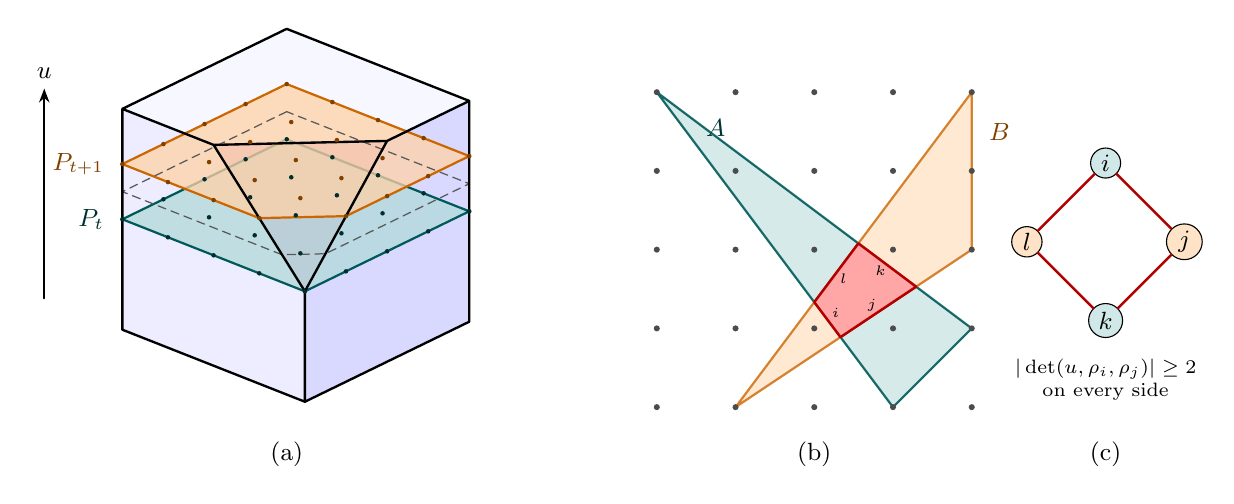
\begin{tikzpicture}[line join=round,line cap=round]
% ---------- (a) the polytope and two slices ----------
\tdplotsetmaincoords{64}{132}
\begin{scope}[tdplot_main_coords,scale=0.78]
  \coordinate (O) at (0,0,0);   \coordinate (X) at (4,0,0);
  \coordinate (Y) at (0,4,0);   \coordinate (XY) at (4,4,0);
  \coordinate (Z) at (0,0,4);   \coordinate (XZ) at (4,0,4);
  \coordinate (YZ) at (0,4,4);
  \coordinate (T1) at (4,4,2);  \coordinate (T2) at (4,2,4); \coordinate (T3) at (2,4,4);
  % hidden edges
  \draw[gray!60,dashed,line width=0.5pt] (O)--(X) (O)--(Y) (O)--(Z);
  % faces
  \fill[blue!7] (X)--(XY)--(T1)--(T2)--(XZ)--cycle;
  \fill[blue!15] (Y)--(XY)--(T1)--(T3)--(YZ)--cycle;
  \fill[blue!3] (Z)--(XZ)--(T2)--(T3)--(YZ)--cycle;
  \fill[violet!30] (T1)--(T2)--(T3)--cycle;
  % the two slices and the half-integral level
  \filldraw[draw=teal!70!black,fill=teal!30,fill opacity=0.75,line width=0.8pt]
     (0,0,2)--(4,0,2)--(4,4,2)--(0,4,2)--cycle;
  \filldraw[draw=orange!80!black,fill=orange!35,fill opacity=0.75,line width=0.8pt]
     (0,0,3)--(4,0,3)--(4,3,3)--(3,4,3)--(0,4,3)--cycle;
  \draw[gray!70!black,densely dashed,line width=0.45pt]
     (0,0,2.5)--(4,0,2.5)--(4,3.5,2.5)--(3.5,4,2.5)--(0,4,2.5)--cycle;
  % visible edges
  \draw[line width=0.85pt] (X)--(XY)--(Y) (X)--(XZ) (Y)--(YZ) (XY)--(T1)
        (Z)--(XZ)--(T2)--(T3)--(YZ)--(Z) (T1)--(T2) (T1)--(T3);
  % lattice points of the two slices
  \foreach \x in {0,...,4}{\foreach \y in {0,...,4}{
     \fill[teal!35!black] (\x,\y,2) circle (1.05pt);}}
  \foreach \x/\y in {0/0,1/0,2/0,3/0,4/0,0/1,1/1,2/1,3/1,4/1,0/2,1/2,2/2,3/2,4/2,
                     0/3,1/3,2/3,3/3,4/3,0/4,1/4,2/4,3/4}{
     \fill[orange!50!black] (\x,\y,3) circle (1.05pt);}
  % labels
  \node[teal!35!black,font=\small,anchor=east] at (4,0,2) {$P_t\ $};
  \node[orange!50!black,font=\small,anchor=east] at (4,0,3) {$P_{t+1}\ $};
  \draw[-{Stealth[length=5pt]},line width=0.7pt] (4.9,-0.9,0.6)--(4.9,-0.9,4.4)
        node[above,font=\small]{$u$};
\end{scope}
\node[font=\small] at (0.0,-2.6) {(a)};
% ---------- (b) the two polygons in the plane ----------
\begin{scope}[xshift=4.7cm,yshift=-2.0cm,scale=1.0]
  \filldraw[draw=teal!70!black,fill=teal!18,line width=0.8pt,opacity=0.9] (0,4)--(3,0)--(4,1)--cycle;
  \filldraw[draw=orange!80!black,fill=orange!22,line width=0.8pt,opacity=0.8] (1,0)--(4,2)--(4,4)--cycle;
  \filldraw[draw=red!70!black,fill=red!35,line width=0.9pt] (2,4/3)--(7/3,8/9)--(56/17,26/17)--(64/25,52/25)--cycle;
  \node[teal!40!black,font=\small] at (0.75,3.55) {$A$};
  \node[orange!50!black,font=\small] at (4.35,3.5) {$B$};
  % side labels
  \node[font=\tiny,inner sep=0pt] at (2.27,1.2) {$i$};
  \node[font=\tiny,inner sep=0pt] at (2.73,1.29) {$j$};
  \node[font=\tiny,inner sep=0pt] at (2.84,1.73) {$k$};
  \node[font=\tiny,inner sep=0pt] at (2.37,1.63) {$l$};
  \foreach \x in {0,...,4}{\foreach \y in {0,...,4}{\fill[black!70] (\x,\y) circle (1.1pt);}}
\end{scope}
\node[font=\small] at (6.7,-2.6) {(b)};
% ---------- (c) the four-cycle in G_u ----------
\begin{scope}[xshift=10.4cm,yshift=0.1cm]
  \node[circle,draw,fill=teal!18,inner sep=1.5pt,font=\small] (i) at (0,1) {$i$};
  \node[circle,draw,fill=orange!22,inner sep=1.5pt,font=\small] (j) at (1,0) {$j$};
  \node[circle,draw,fill=teal!18,inner sep=1.5pt,font=\small] (k) at (0,-1) {$k$};
  \node[circle,draw,fill=orange!22,inner sep=1.5pt,font=\small] (l) at (-1,0) {$l$};
  \draw[red!70!black,line width=0.9pt] (i)--(j)--(k)--(l)--(i);
  \node[font=\scriptsize,align=center] at (0,-1.75) {$|\det(u,\rho_i,\rho_j)|\ge 2$\\ on every side};
\end{scope}
\node[font=\small] at (10.4,-2.6) {(c)};
\end{tikzpicture}
\end{document}
